\documentclass[12pt,a4paper]{article}

\usepackage{caption}
\usepackage{subcaption}
\usepackage{tabularx}
\usepackage{graphicx}
\usepackage{amsfonts} 
\usepackage{amssymb}
\usepackage{amsmath}
\usepackage[a4paper,margin=4cm]{geometry}
\usepackage{indentfirst}
\usepackage{lastpage}
\usepackage{wrapfig}
\usepackage[colorlinks = true,
            linkcolor = blue,
            urlcolor  = blue]{hyperref}
\usepackage{listings}

\newcommand{\changeurlcolor}[1]{\hypersetup{urlcolor=#1}}   

\usepackage{awesomebox}
\usepackage{fancyhdr}

\usepackage[australian]{babel}
\usepackage{datetime}

\newcommand{\titlestr}{Optimistic Lock-Based List-Based Set Implementations Project Report}
\newcommand{\authorstr}{Phuc Lai Le}

\begin{document}
\begin{titlepage}
  \centering
  \includegraphics[width=0.3\textwidth]{tplogo.png}

  \vspace{1cm}
  {\LARGE \bf{\titlestr} \par}
  
  \vspace{.5cm}
  {\LARGE {\it{Distributed algorithms (Part A)} \\ (CSC\_4SL05\_TP)} \par}

  \vspace{1cm}
  {\Large \authorstr \par}

  \vspace{1cm}

  \today

  \vfill
\end{titlepage}

\newpage

{
  \hypersetup{linkcolor=black}
  \tableofcontents
}

\newpage
\section{Implementations of the hand-over-hand algorithm}
\subsection{Java code}
The Java code for the implementations of the hand-over-hand algorithm is described below:

\begin{lstlisting}[language=Java]
package linkedlists.lockbased;

import java.util.concurrent.locks.Lock;
import java.util.concurrent.locks.ReentrantLock;

import contention.abstractions.AbstractCompositionalIntSet;

public class HandOverHand extends AbstractCompositionalIntSet {
    private Node head;
    private Node tail;

    public HandOverHand(){
        head = new Node(Integer.MIN_VALUE);
        tail = new Node(Integer.MAX_VALUE);
        head.next = tail;
    }

    @Override
    public boolean addInt(int item) {
        head.lock();
        Node pred = head;
        try {
            Node curr = pred.next;
            curr.lock();

            try {
                while (curr.key < item) {
                    pred.unlock();
                    pred = curr;
                    curr = curr.next;
                    curr.lock();
                }

                if (curr.key == item) {
                    return false;
                }

                Node newNode = new Node(item);
                newNode.next = curr;
                pred.next = newNode;
                return true;
            } finally {
                curr.unlock();
            }
        } finally {
            pred.unlock();
        }
    }

    @Override
    public boolean removeInt(int item) {
        head.lock();
        Node pred = head;
        Node curr = pred.next;
        try {
            curr.lock();
            try {
                while (curr.key < item) {
                    pred.unlock();
                    pred = curr;
                    curr = pred.next;
                    curr.lock();
                }
                if (curr.key == item) {
                    pred.next = curr.next;
                    return true;
                }
                return false;
            } finally {
                curr.unlock();
            }
        } finally {
            pred.unlock();
        }
    }

    @Override
    public boolean containsInt(int item) {
        head.lock();
        Node pred = head;
        Node curr = pred.next;
        try {
            curr.lock();
            try {
                while (curr.key < item) {
                    pred.unlock();
                    pred = curr;
                    curr = pred.next;
                    curr.lock();
                }
                return (curr.key == item);
            } finally {
                curr.unlock();
            }
        } finally {
            pred.unlock();
        }
    }
    
    @Override
    public int size() {
        int count = 0;

        Node curr = head.next;
        while (curr.key != Integer.MAX_VALUE) {
            curr = curr.next;
            count++;
        }
        return count;
    }

    @Override
    public void clear() {
       head = new Node(Integer.MIN_VALUE);
       head.next = new Node(Integer.MAX_VALUE);
    }

    private class Node {
        private Lock lock = new ReentrantLock();

        public int key;
        public Node next;

        Node(int item) {
            key = item;
            next = null;
        }

        void lock(){
            this.lock.lock();
        }

        void unlock(){
            this.lock.unlock();
        }
    }
}
\end{lstlisting}

\subsection{Proofs of the algorithm}
\subsubsection{Safety}
For all of the operation, consider the linearization point is the moment when the locks are established. 

More specifically, the linearization point for \textit{insert(item)} operation is when the node with the next higher key is locked (the call is successful and returns true) or when the node that contains \textit{item} is locked (the call is unsuccessful and returns false).

For \textit{remove(item)}, the linearization point of this operation for successful call are the moment when the predecessor node is locked if \textit{item} is in the list, or when the node containing the next higher key is locked if \textit{item} is not in the list. The linearization point for unsuccessful call is when the node containing \textit{item} is locked if \textit{item} is in the list.

For \textit{contains(item)} operation, the linearization point is when the node that contains \textit{item} is locked if \textit{item} is in the list, or when the node containing the next higher key is locked if \textit{item} is not in the list.

Because the \textit{pred} and \textit{curr} nodes is locked during the phase when the operation makes changes, they cannot be remove or update by others processes until the locks are released. Only one process can access them at a time. Therefore, the structure of the node is preserved and the data consistency of the list is maintained.

\subsubsection{Liveness}
Because the locks are acquired in a sequential manner, deadlock or starvation will not happen. A process hold the lock of the current node before acquiring the lock of the next node. This prevents other processes from interfering with the current process's progress.

The operations acquire locks by traversing down the list manner. Because there are no deadlocks, the process which is ahead on the list will be able to make progress, by modifying the node that it is locking or continue to traverse down the list as the following node is not locked. Eventually, all the locks that is held by that process will be released, and the process that is behind will be able to acquire the locks and make progress also. Assuming the list is finite and because the processes will always make progress, a process will eventually reach the end of the list.

\newpage
\section{Performance Analysis}
\subsection{Fixed update ratio 10\% and list size 1000}
For this experiment, the three algorithms, Coarse-grained, Hand-over-hand and Lazy Linked List will be ran through synchrobench with the fixed update ratio of 10\% and list size of 1000. The number of threads is increased after each run for each algorithm and the results is described below:

\begin{figure}[h]
    \centering
    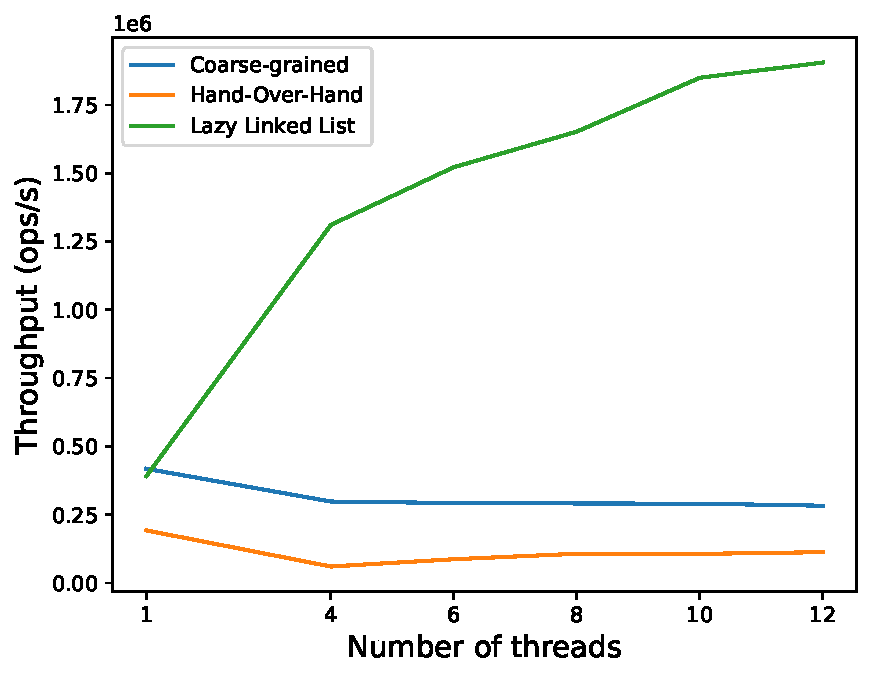
\includegraphics[width=0.75\textwidth]{fixed_update_listsize.pdf}
    \caption{Throughput of the algorithms with fixed update ratio and list size}
    \label{fig:fixed_update_listsize}
\end{figure}

Overall, the Lazy Linked List algorithm performs best across all thread counts, then the Coarse-grained algorithm, and the Hand-over-hand algorithm perform worse. 

For the Lazy Linked List algorithm, the good performance came from the wait-free approach. Therefore, the overhead of locking is avoided. This algorithm also has a excellent scalability, as its performance continue to improve with increasing numbers of threads.

For the Coarse-grained algorithm, throughput is relatively low and remains almost constant as the number of threads increases. This is because the algorithm uses a single global lock to protect the entire list. When multiple threads contend for this lock, they are forced to wait. 

For the Hand-over-hand algorithm, as the number of threads increase, the throughput also increase This is because of the fine-grained locking that it uses. This reduces contention and allows multiple threads to access different parts of the list concurrently. However, the algorithm eventually hits a performance plateau. This is due to the overhead introduced by managing the locks. The more the number of threads, the more the overhead becomes more significant, limiting further performance gains. The performance of Hand-over-hand algorithm is worst in the three. Theoretically, this algorithm allows more parallelism, which leads to the increment of efficiency. This results could be from the overhead by the locks, which likely outweighs the potential efficiency gains, especially at higher thread counts.

\subsection{Fixed list size 1000}
For this experiment, the three algorithms, Coarse-grained, Hand-over-hand and Lazy Linked List will be ran through synchrobench with the fixed list size of 1000 and varying update ratio (0\%, 10\%, 100\%).

\subsubsection{Coarse-grained}
\begin{figure}[h]
    \centering
    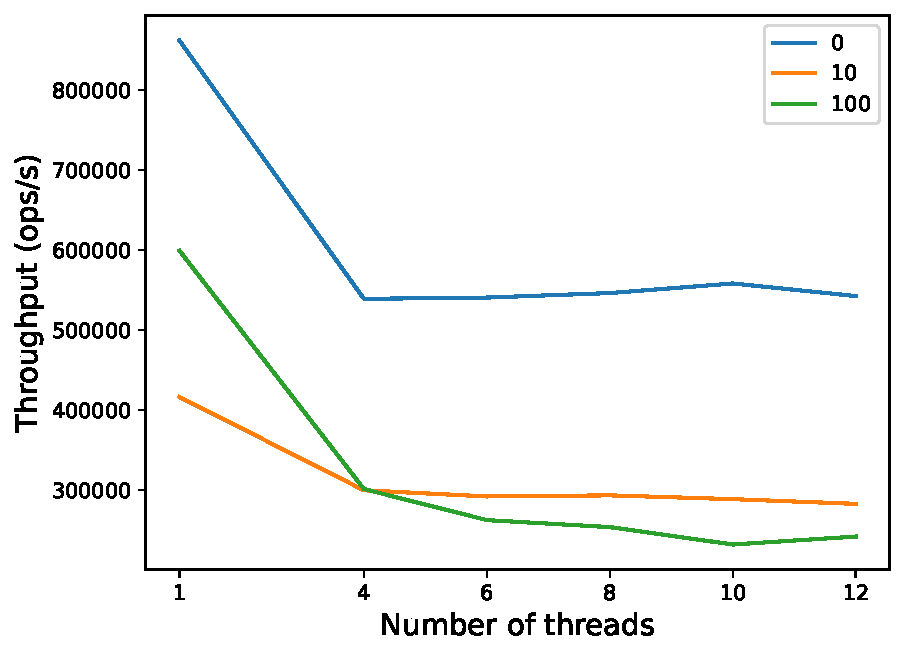
\includegraphics[width=0.75\textwidth]{fixed_listsize_coarse_grained.pdf}
    \caption{Throughput of Coarse-grained algorithm with varying update ratio}
    \label{fig:fixed_update_coarse_grained}
\end{figure}

The overall trend for all three curve is going downward. As the number of threads increases, the throughput generally decreases for all update ratios. This is because of coarse-grained locking where a single lock protects the entire list. When multiple threads contend for this lock, they have to wait, leading to performance degradation.

The update ratio has impact on the throughput of the algorithm. With no update (0\% update ratio), the algorithm only performs read operation, therefore performs best. As the update ratio increases (10\% update ratio), the contention for the lock also increases. This leads to a more significant drop in throughput as the number of threads grows. With all operations being updates (100\% update ratio), the contention for the lock is highest. This results in the most significant decrease in throughput as the number of threads increase.

In conclusion, throughput is inversely related to the update ratio. Write-intensive workloads lead to more contention for the lock, reducing throughput. The algorithm also does not scale well when the number of threads increase.

\subsubsection{Hand-over-hand}
\begin{figure}[h]
    \centering
    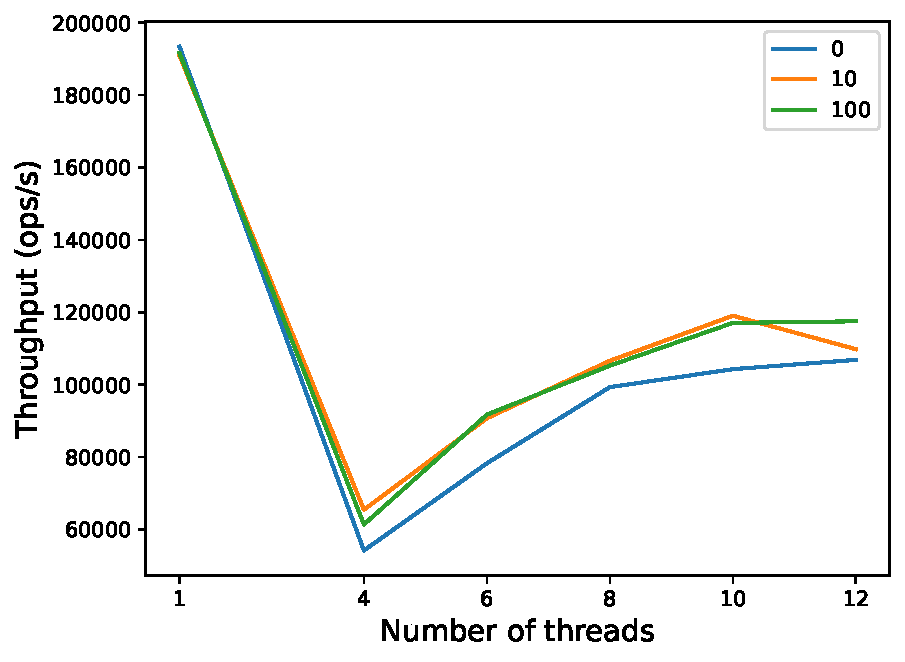
\includegraphics[width=0.75\textwidth]{fixed_listsize_hands_over_hands.pdf}
    \caption{Throughput of Hand-over-hand algorithm with varying update ratio}
    \label{fig:fixed_listsize_hands_over_hands}
\end{figure}

For all update ratios, throughput starts relatively high with one thread but drops significantly as the number of threads increases to 4. This drop is likely due to the overhead associated with managing the locks. But after the initial drop, throughput begins to increase again as the thread count rises, reaching a relatively stable level between 8 and 12 threads. This suggests that after the initial lock management overhead, the hand-over-hand locking begins to take advantage of increased parallelism with more threads. Around 8–12 threads, there are less increment and even a decrease in performance with the case of 10\% update ratio. This indicates that there exits a point of balance where adding more threads does not significantly improve throughput because of contention and lock overhead.

The performance differences between the three update ratios (0\%, 10\%, and 100\%) are relatively small. This is because, with hand-over-hand locking, each thread locks nodes individually, which introduce similar overhead for both read and write operations.

\subsubsection{Lazy Linked List}
\begin{figure}[h]
    \centering
    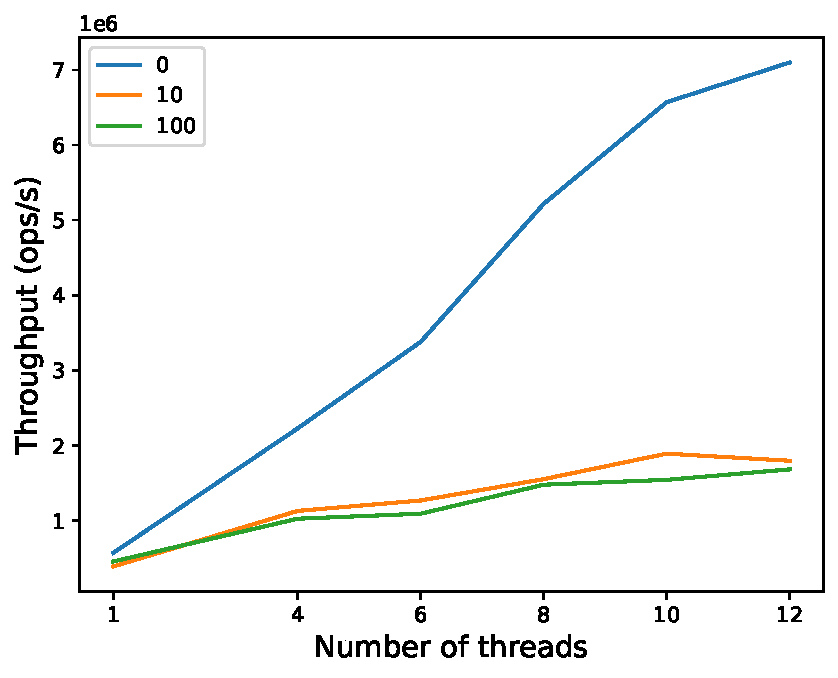
\includegraphics[width=0.75\textwidth]{fixed_listsize_lazy_linked_list.pdf}
    \caption{Throughput of Lazy Linked List algorithm with varying update ratio}
    \label{fig:fixed_listsize_lazy_linked_list}
\end{figure}

As the number of threads increases, the throughput generally increases for all update ratios. This is because the algorithm allows threads to proceed without locking and only locking when necessary, resulting in minimizes contention. 

With no update (0\% update ratio), the algorithm only performs read operation and has the best results. Since there are no updates, the algorithm benefits from minimal locking, allows more threads to operate on the list concurrently. With the increment in update ratio (10\% update ratio), some locking for updates is introduced, therefore reduce the concurrency. With all operations being updates (100\% update ratio), throughput is the lowest in this scenario. In a write-only workload, each operation requires locking, which increases contention, leads to a decrease in throughput.

\subsection{Fixed update ratio 10\%}
For this experiment, the three algorithms, Coarse-grained, Hand-over-hand and Lazy Linked List will be ran through synchrobench with the fixed update ratio 10\% and varying list size (100, 1000, 10000). In some cases, to able to see the trend of a curve, a subplot is included.

\subsubsection{Coarse-grained}
\begin{figure}[h]
    \centering
    \subfloat[\centering]{{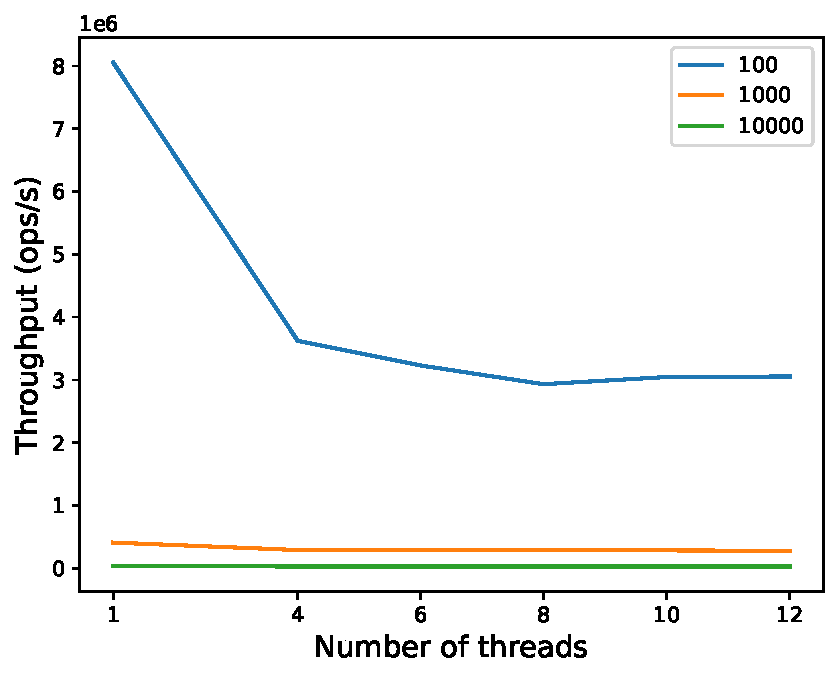
\includegraphics[width=0.45\textwidth]{fixed_update_coarse_grained.pdf} }}
    \qquad
    \subfloat[\centering]{{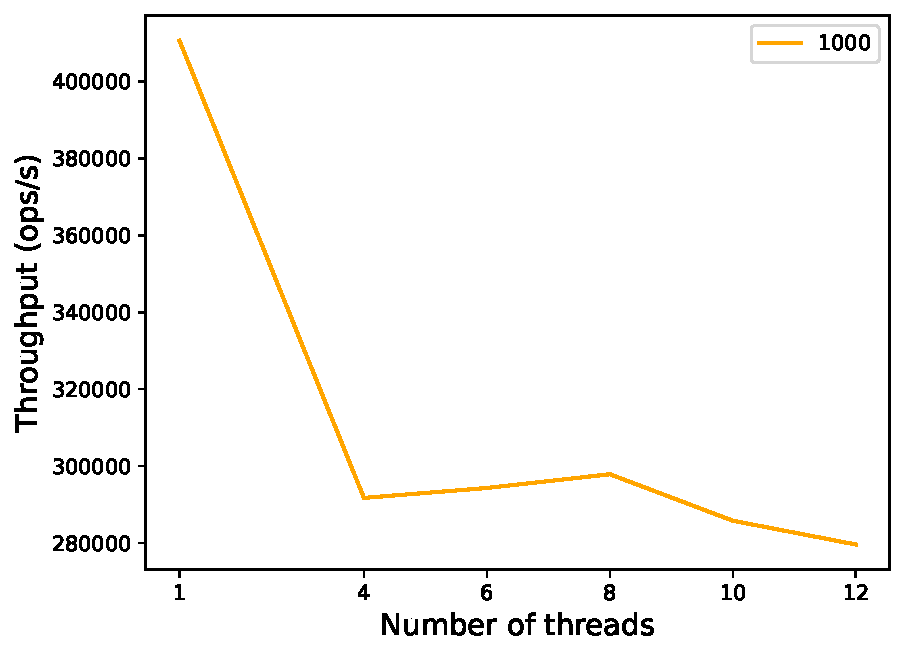
\includegraphics[width=0.45\textwidth]{fixed_update_coarse_grained_1000.pdf} }}
    \qquad
    \subfloat[\centering]{{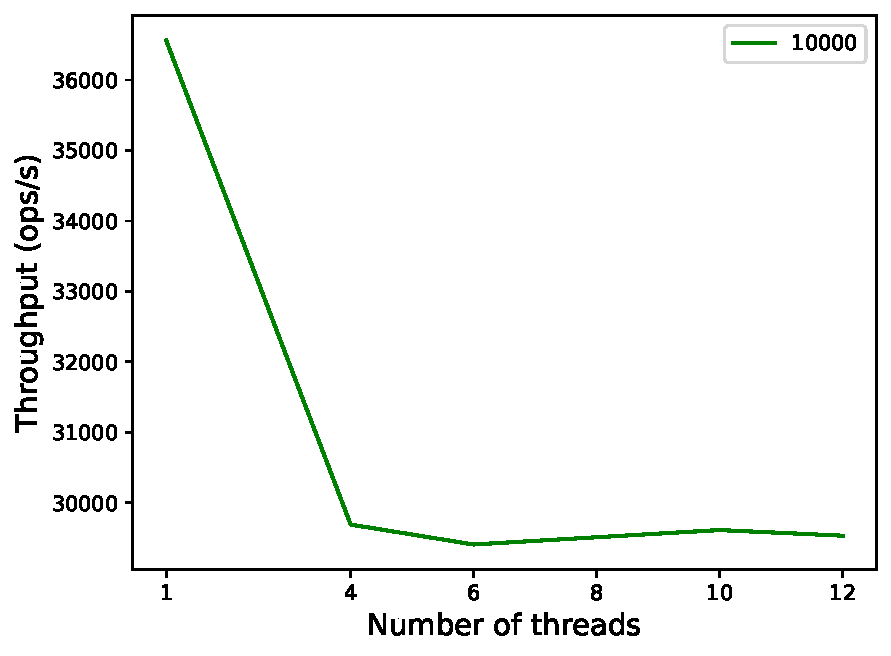
\includegraphics[width=0.45\textwidth]{fixed_update_coarse_grained_10000.pdf} }}
    \caption{hroughput of Coarse-grained algorithm with varying list size}%
    \label{fig:fixed_update_coarse_grained}%
\end{figure}

The characteristic of Coarse-grained algorithm is still displayed in the results. As the number of threads increases, the throughput generally decreases for all list sizes and the algorithm does not scale well due to the high contention. Once the number of threads reaches 4, throughput stabilizes or slightly declines.

With the list size of 100, throughput is initially high with 1 thread but drops sharply as the number of threads increases to 4 and after that, the throughput stabilizes. The similar pattern applies for the others cases. As the list size increases, the overall throughput becomes lower. This is due to the time to traverse the list increases significantly as the list grows larger. 

\subsubsection{Hand-over-hand}
\begin{figure}[h]
    \centering
    \subfloat[\centering]{{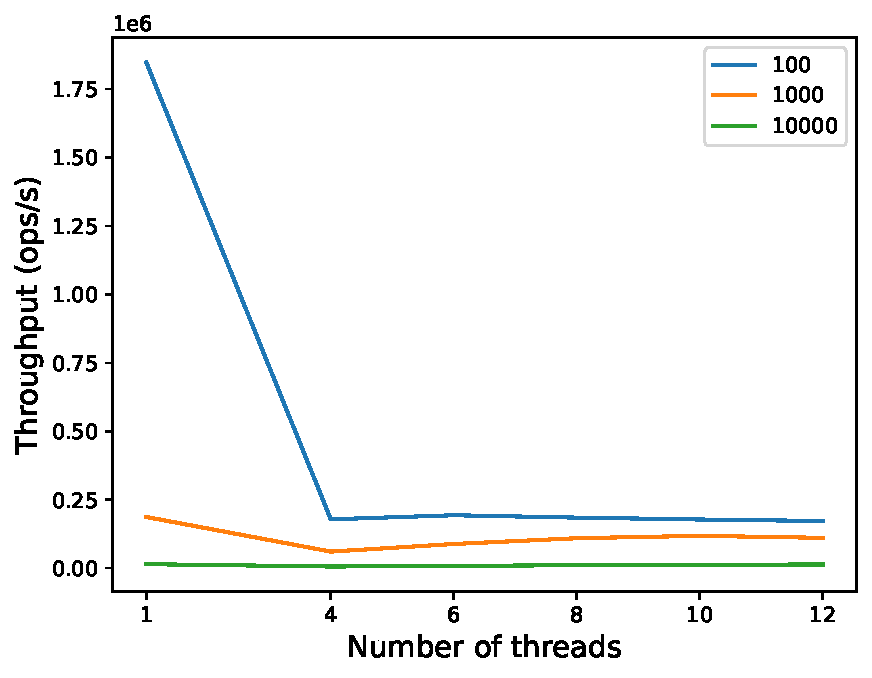
\includegraphics[width=0.45\textwidth]{fixed_update_hands_over_hands.pdf} }}
    \qquad
    \subfloat[\centering]{{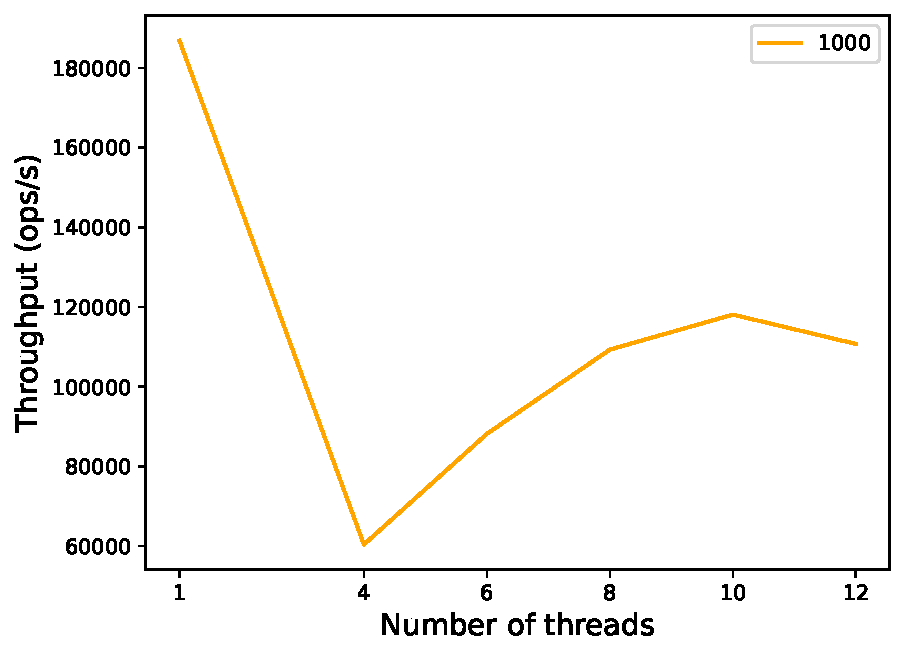
\includegraphics[width=0.45\textwidth]{fixed_update_hands_over_hands_1000.pdf} }}
    \qquad
    \subfloat[\centering]{{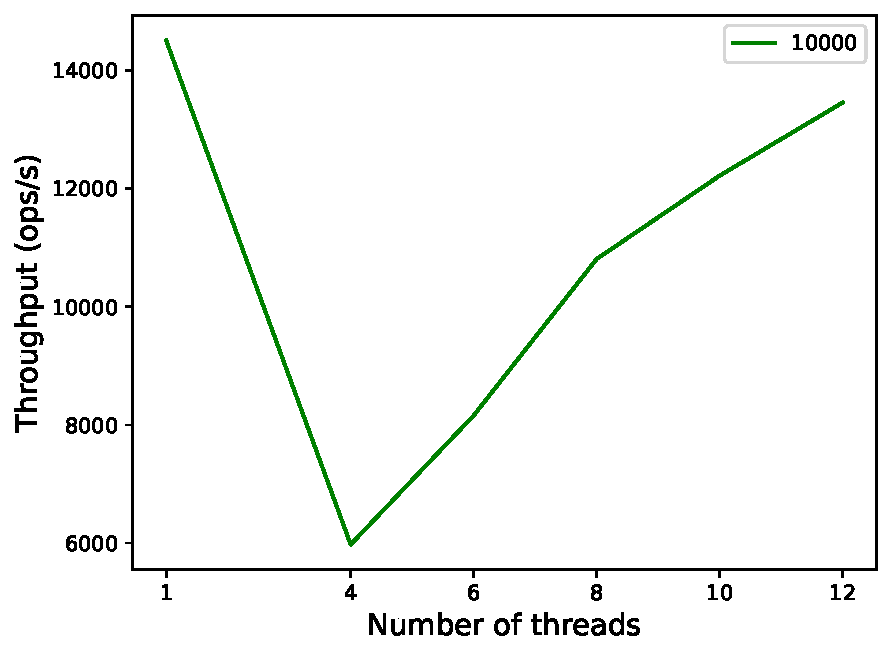
\includegraphics[width=0.45\textwidth]{fixed_update_hands_over_hands_10000.pdf} }}
    \caption{Throughput of Hand-over-hand algorithm with varying list size}%
    \label{fig:fixed_update_hand_over_hand}%
\end{figure}

The results show the overall trend similar to the case of fixed list size. Throughput is high with a single thread, then drops sharply at 4 threads, due to the introduction of overhead of locks management, then continue to increase as the number of threads grow. The algorithm has better scalability compare to Coarse-grained algorithm, can handle high levels of concurrency.

With a fixed update ratio, the algorithm performs best when the list size is smaller, in this case is when the list size is only 100. The decrease of performance appears when the list size increase. This could be a result of reduced traversal and locking overhead when the list size is smaller.

\subsubsection{Lazy Linked List}
\begin{figure}[h]
    \centering
    \subfloat[\centering]{{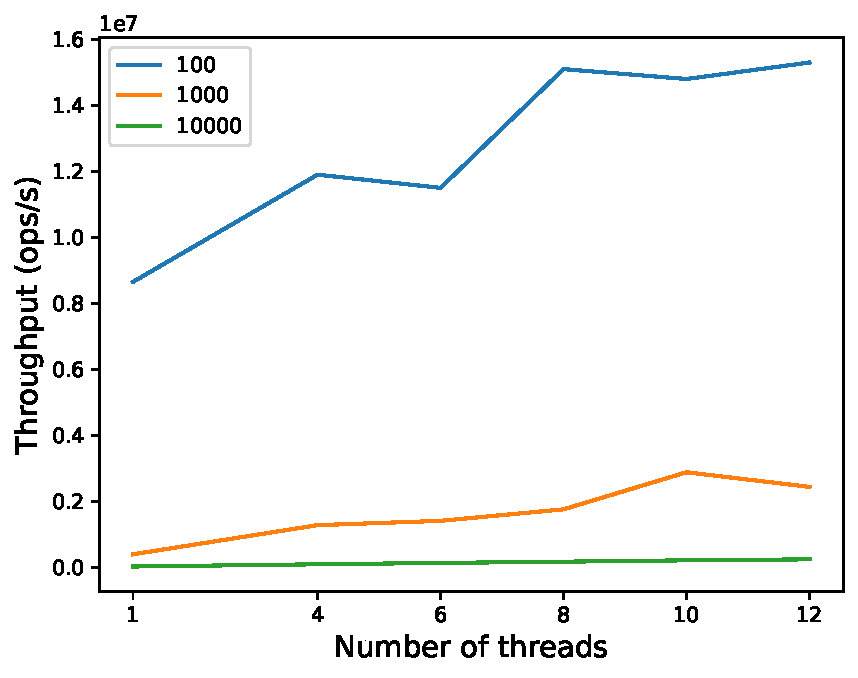
\includegraphics[width=0.45\textwidth]{fixed_update_lazy_linked_list.pdf} }}
    \qquad
    \subfloat[\centering]{{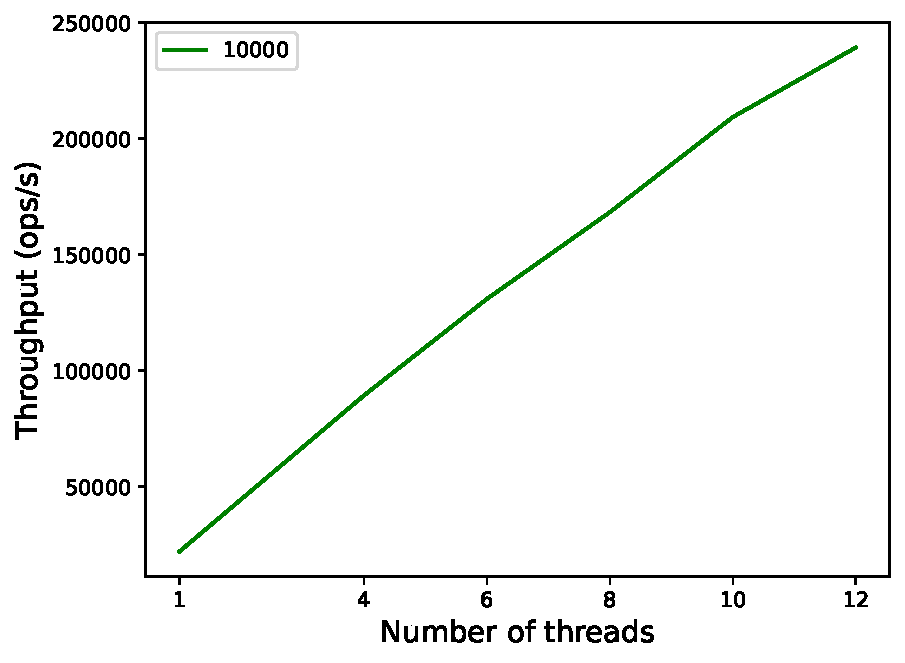
\includegraphics[width=0.45\textwidth]{fixed_update_lazy_linked_list_10000.pdf} }}
    \caption{Throughput of Lazy Linked List algorithm with varying list size}%
    \label{fig:fixed_update_lazy_linked_list)}%
\end{figure}

For the overall trend, as the number of threads increases, the throughput generally increases for all list sizes, demonstrates  a good scalability. This is a characteristic of this algorithm, as described in the results above. 

The throughput is high with smaller list size, and decrease when the list size increase. Similar to Hand-over-hand algorithm, this could be a result of less traversal time with smaller list. 

\newpage
\section{Appendix}
\subsection{Machine's system details}
\begin{tabularx}{0.8\textwidth} { 
  | >{\raggedright\arraybackslash}X 
  | >{\centering\arraybackslash}X 
  | >{\raggedleft\arraybackslash}X | }
 \hline
 name & lame24.enst.fr \\
  \hline
 Linux distro & Ubuntu 24.04.1 LTS \\
 \hline
 Kernel & 6.8.0-47-generic \\
 \hline
 Threads & 96 \\
 \hline
 Java version  & openjdk version "21.0.4" 2024-07-16
 
OpenJDK Runtime Environment (build 21.0.4+7-Ubuntu-1ubuntu224.04)

OpenJDK 64-Bit Server VM (build 21.0.4+7-Ubuntu-1ubuntu224.04, mixed mode, sharing)
 \\
\hline
\end{tabularx}

\subsection{Source code}

\end{document}

